% !TeX root = ../Thesis.tex

\chapter{Introduction}

%Classical lasers, such as a laser pointer or a Helium-Neon gas laser, are limited to a single wavelength since the light is generated by stimulated emission. Tuneable lasers on the other hand, have the ability to operate within a range of wavelengths \cite{bohun, burgoyne2010, yamashita}. As a result, tuneable lasers have applications in spectroscopy and high resolution imaging such as coherent anti-Stokes Raman spectroscopy and optical coherence tomography \cite{bohun, burgoyne2014, yamashita}. This article is concerned with dispersion-tuned actively mode-locked (DTAML) lasers. The laser cavity consists of four elements: the dispersive element, the modulator, the gain fibre, and the optical coupler. The gain fibre consists of either an Erbium or Ytterbium doped fibre, and dispersion is generated by the highly dispersive chirped fibre Bragg grating (CFBG). \\

\section{Tuneable Lasers}
\begin{figure}[htbp]
\centering
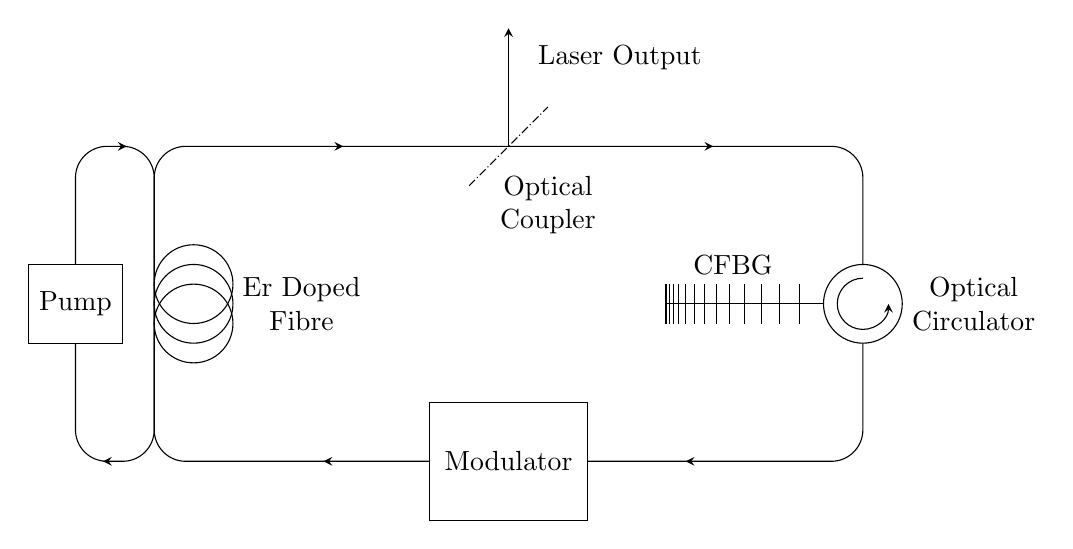
\begin{tikzpicture}
% Two laser loops
\draw [rounded corners=4mm] (0,0) rectangle ++(9,4);
\draw [rounded corners=4mm] (0,0) rectangle ++(-1,4);

% Gain
\draw (0.5,2.25) circle (0.5cm);
\draw (0.5,2) circle (0.5cm) node [anchor=west,xshift=0.5cm,align=center] {Er Doped \\ Fibre};
\draw (0.5,1.75) circle (0.5cm);

% Modulator and pump
\filldraw[fill=white, draw=black] (3.5,-0.75) rectangle ++(2,1.5) node [midway] {Modulator};
\filldraw[fill=white, draw=black] (-1.6,1.5) rectangle ++(1.2,1) node [midway] {Pump};

% Coupler and output
\draw[-stealth] (4.5,4) -- (4.5,5.5) node [pos=0.75,anchor=west,xshift=0.25cm] {Laser Output};
\draw[densely dashdotted] (4,3.5) -- (5,4.5) node [pos=1,anchor=north,yshift=-0.75cm,align=center] {Optical \\ Coupler};

% Circulator
\filldraw[fill=white, draw=black] (9,2) circle (0.5cm) node [anchor=west,xshift=0.5cm,align=center] {Optical \\ Circulator};
\draw[->,>=stealth] (9,2.325) arc (90:360:0.325cm);

% Grating
\draw (8.5,2) -- (6.5,2) node [pos=0.5,anchor=south,yshift=0.25cm,xshift=-0.15cm] {CFBG};
\foreach \i in {0,...,13}
  \draw (6.5 + \i*\i/100,1.75) -- (6.5 + \i*\i/100,2.25);

% Arrows
\draw[-stealth] (2.16,0) -- (2.15,0);
\draw[-stealth] (2.39,4) -- (2.4,4);
\draw[-stealth] (6.76,0) -- (6.75,0);
\draw[-stealth] (7.09,4) -- (7.1,4);
\draw[-stealth] (-0.649,0) -- (-0.65,0);
\draw[-stealth] (-0.351,4) -- (-0.35,4);H
\end{tikzpicture}
\caption[Laser Cavity]{Laser cavity schematic.}
\label{fig:cavity}
\end{figure}

\subsection{Optical Coupler and Laser Output}
The optical coulper is a device that splits its input into two outputs---one continuing through the laser cavity, while the other exits the cavity to become the output of the laser. There are multiple devices that can accomplish this, however, the simplest is a partially reflecting mirror \cite{alazzawi}. These mirrors are characterized by their reflection coefficient, $R$. In the schematic shown in Figure \ref{fig:cavity}, the part of the signal that is reflected exits the cavity, whereas, the part of the signal transmitted remains within the cavity. \\

\subsection{Modulator}

\subsection{Fibre Bragg Grating}
A fibre Bragg grating (FBG) is an optical fibre where the refractive index varies periodically along its length \cite{ferreira}. To achieve this, typically silica fibres are doped with Germanium, which when exposed to intense ultraviolet (UV) light alters the refractive index of the core \cite{becker, starodoumov}. The photosensitivity of the optical fibres can be increased by more than an order of magnitude by the Germanium doping \cite{becker, ferreira}. \\

\begin{figure}[p]
\centering
\begin{subfigure}{\textwidth}
\centering
% !TeX root = ../Thesis.tex

\begin{tikzpicture}
\draw[pattern=north east lines, pattern color=blue] (-4,0.5) rectangle (4,1); % Top Insulation
\draw[pattern=north west lines, pattern color=blue] (-4,-0.5) rectangle (4,-1); % Bottom Insulation
\draw[pattern=mydots, pattern color=OliveGreen] (-4,-0.5) rectangle (4,0.5); % Core
\draw[fill=black] (-2,1.5) rectangle (2,1.75); % Phase Mask top

\foreach \i in {0,...,7}
  \draw[magenta, thick] (-1.75 + \i/2,5) -- (-1.75 + \i/2,1.5);

\foreach \i in {0,...,3}{
  % Phase mask teeth
  \draw[fill=black] (-2 + \i,1.25) rectangle (-1.75 + \i,1.5); 
  \draw[fill=black] (-1.25 + \i,1.25) rectangle (-1 + \i,1.5);
  % Rays
  \draw[->, >=stealth, magenta, thick] (-1.75 + \i,1.5) -- (-1.25 + \i,-1.5);
  \draw[->, >=stealth, magenta, thick] (-1.25 + \i,1.5) -- (-1.75 + \i,-1.5);
}
% Labels
\draw[->, >=stealth, thick] (3,-1.5) -- (2,0) node[pos=-0.2] {Ge-Doped Core};
\draw[->, >=stealth, thick] (-3,-1.5) -- (-2,-0.75) node[pos=-0.3] {Cladding};
\draw[->, >=stealth, thick] (-3,2.5) -- (-1.75,2) node[pos=-0.4] {UV Light};
\draw[->, >=stealth, thick] (3,2.5) -- (2,1.5) node[pos=-0.2] {Phase-Mask};
\end{tikzpicture}
\caption{\textbf{Phase-Mask:} The phase-mask refracts the UV light onto the core.}
\label{fig:phasemask}
\vspace{10mm}
\end{subfigure}
\begin{subfigure}{\textwidth}
\centering
% !TeX root = ../Thesis.tex

\begin{tikzpicture}

\draw[pattern=north east lines, pattern color=blue] (-4,0.5) rectangle (4,1); % Top Insulation
\draw[pattern=north west lines, pattern color=blue] (-4,-0.5) rectangle (4,-1); % Bottom Insulation
\draw[pattern=mydots, pattern color=OliveGreen] (-4,-0.5) rectangle (4,0.5); % Core

\foreach \i in {0,...,3}{
  % Rays
  \draw[->, >=stealth, magenta, thick] (-2.25 + \i,4.5) -- (-1.25 + \i,-1.5);
  \draw[->, >=stealth, magenta, thick] (-0.75 + \i,4.5) -- (-1.75 + \i,-1.5);
}
% Labels
\draw[->, >=stealth, thick] (3,-1.5) -- (2,0) node[pos=-0.2] {Ge-Doped Core};
\draw[->, >=stealth, thick] (-3,-1.5) -- (-2,-0.75) node[pos=-0.3] {Cladding};
\draw[->, >=stealth, thick] (-3,2.5) -- (-1.82,2) node[pos=-0.4] {\gls{uv} Light};
\end{tikzpicture}
\caption{\textbf{Holographic Side Exposure:} Two incident beams intersect at the core.}
\label{fig:holographic}
\end{subfigure}
\caption{Depictions of the two methods for manufacturing FBGs. The UV light is focused on the core causing periodic constructive and destructive interference.}
\label{fig:fbgmake}
\end{figure}

FBGs are manufactured using one of two methods---the phase-mask method \cite{agrawal2002, alazzawi, becker, starodoumov}, or the holographic side exposure method \cite{agrawal2002, alazzawi, becker, ferreira, starodoumov}---these are shown in Figure \ref{fig:fbgmake}. Both methods cause the periodic nature of the refractive index through interference. In the phase-mask method (Figure \ref{fig:phasemask}) a single beam of UV light passes through the phase-mask which acts as a series of lenses, focusing the light at the core---this causes a sinusoidal interference pattern. Similarly, in the holographic side exposure method (Figure \ref{fig:holographic}), two beams of UV light are instead used to create the interference pattern. \\

The purpose of FBGs is that they act as reflective filters \cite{agrawal2002, alazzawi, ferreira, starodoumov}. Due to the periodicity of the refractive index, light with the corresponding wavelength will be reflected with all others passing through. This wavelength is defined by the Bragg condition \cite{agrawal2002, alazzawi, becker, ferreira, silfvast, starodoumov}:
\begin{align}
\label{eq:bragg}
\lambda_B = 2 \Lambda \bar{n},
\end{align}
where $\lambda_B$ is the Bragg wavelength, $\Lambda$ is the period of the grating, and $\bar{n}$ is the average index of refraction. This reflects wavelengths close to $\lambda_B$, known as the stop-band. \\

\subsubsection{Chirped Fibre Bragg Grating}
\begin{figure}[tbp]
\begin{subfigure}{0.5\textwidth}
\input{./Figures/Unchirped}
\caption{Unchirped Gaussian pulse.}
\label{fig:unchirped}
\end{subfigure}
\begin{subfigure}{0.5\textwidth}
\input{./Figures/Chirped}
\caption{Linearly chirped Gaussian pulse.}
\label{fig:chirped}
\end{subfigure}
\caption{In a unchirped pulse the frequency is constant, however, in a chirped pulse the frequency varies along the envelope.}
\label{fig:chirp}
\end{figure}

Chirp is simply the term for a signal that has a non-constant frequency across it. Figure \ref{fig:chirp} shows examples of chirped and unchirped Gaussian pulses---the most common type of chirp is linear chirp, where the frequency varies linearly across the pulse. Because of this, the oscillations are characterized by $\exp \left( i C x^2 \right)$, where $C x$ is the linear variation of the wave number, and $C$ is the chirp parameter. By using a chirped phase-mask a chirped fibre Bragg grating (CFBG) can be created. Since the period of the refractive index varies across the CFBG, so does when the Bragg condition, \eqref{eq:bragg}, is satisfied. This causes most wavelengths to be reflected by a CFBG, but with each wavelength penetrating to a different depth. A consequence of this is that a time delay is created between wavelengths---this is depicted in Figure \ref{fig:cfbg} with the upper portion showing  the refractive index as a function of the depth. In this orientation, the red (dashed) wave is unable to penetrate as far as the blue (solid) wave since each wave is reflected where it matches the frequency of the refractive index.  \\

\begin{figure}[tbp]
\centering
% !TeX root = ../Thesis.tex

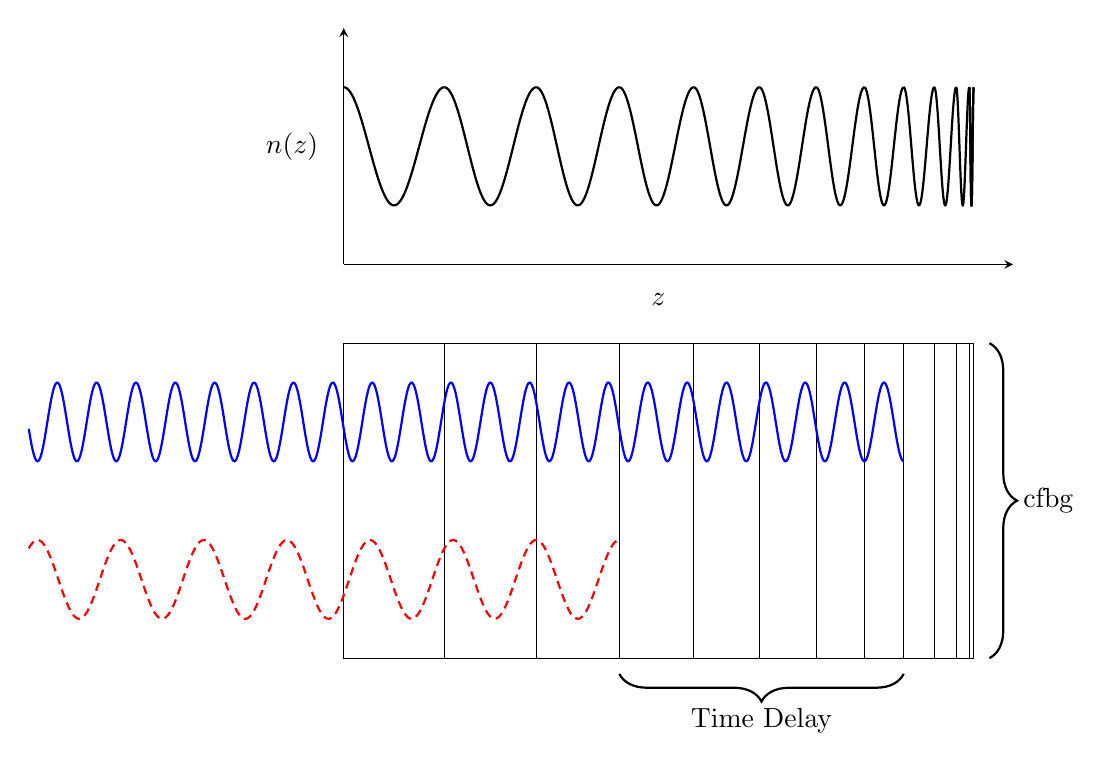
\begin{tikzpicture}
% CFBG
\draw (4,0) -- (12,0) -- (12,4) -- (4,4) -- cycle;
\foreach \i in {1,...,12}
  \draw (12 - 1/18*\i*\i,0) -- (12 - 1/18*\i*\i,4);
%\foreach \i in {0,...,12}
%  \draw [dashed] (12 - 1/18*\i*\i,4) -- (12 - 1/18*\i*\i,8);
% Waves
\draw [domain=0:(12-16/18), samples=1000, blue, thick] plot (\x, {-0.5*cos(4*pi*(\x-(12-25/18)) r) + 3});
\draw [domain=0:(12-81/18), samples=500, red, thick, densely dashed] plot (\x, {0.5*cos(2*pi*36/38*(\x-(12-100/18)) r) + 1});

% Labels
\draw [thick, decorate, decoration={brace, mirror, raise=0.2cm, amplitude=10pt}] (7.5,0) -- (100/9,0)
node [pos=0.5,anchor=north,yshift=-0.5cm] {Time Delay};
\draw [thick, decorate, decoration={brace, mirror, raise=0.2cm, amplitude=10pt}] (12,0) -- (12,4)
node [pos=0.5,anchor=west,xshift=0.5cm] {\gls{cfbg}};

% Index of refraction
\draw [->, >=stealth] (4,5) -- (12.5,5)
node [pos=0.47,anchor=north,yshift=-0.25cm] {$z$};
\draw [->, >=stealth] (4,5) -- (4,8)
node [pos=0.5,anchor=east,xshift=-0.2cm] {$n(z)$};
\foreach \i in {0,...,12}
  \draw [domain=(12-\i*\i/18):(12-(\i-1)*(\i-1)/18), samples=100, black, thick] plot (\x, {3/4*cos(2*pi*36/(4*\i-2)*(\x-(12-\i*\i/18)) r) + 6.5});
\end{tikzpicture}
\caption[CFBG]{CFBG}
\label{fig:cfbg}
\end{figure}

The speed of light in an optical fibre is slightly dependent on the wavelength---this causes light with a longer wavelength to travel faster, and is known as chromatic dispersion. This is a large problem in fibre optic communications, the signal can spread and potentially becomes uninterpretable after large distances. However, chromatic dispersion can be counteracted using a CFBG \cite{agrawal2002, alazzawi, becker, starodoumov} (in the opposite orientation of Figure \ref{fig:cfbg}). By forcing the longer wavelengths to travel farther the dispersion can be reversed, restoring the original signal. In one experiment \cite{dong}, a signal was successfully transmitted over $109$ km at $40$ Gb/s by compensating the dispersion with two  $40$ cm CFBGs. Over this distance, the pulse would have spread to about $55$ times its original width, and could only have been transmitted $4$ km at that bit rate. At reduced bit rates however, a $10$ cm CFBG can compensate the dispersion of $300$ km of fibre \cite{agrawal2002}. However, in our case, we wish to accelerate the dispersion, simulating hundreds of metres of fibre, so the CFBG is used in the orientation shown in Figure \ref{fig:cfbg}. \\

\subsection{Optical Circulator}
\begin{wrapfigure}{O}{0.5\textwidth}
\centering
% !TeX root = ../Thesis.tex

\begin{tikzpicture}
%Fibres
\draw (-2.25,0) -- (2.25,0);
\draw (0,2.25) -- (0,-2.25);

% Circulator
\filldraw[fill=white] (0,0) circle (1);
\draw[->,>=stealth] (0,0.65) arc (90:360:0.65);

%Labels
\node at (0.25, 1.5){$1$};
\node at (-1.5, 0.25){$2$};
\node at (-0.25, -1.5){$3$};
\node at (1.5, -0.25){$4$};
\end{tikzpicture}
\caption[Optical Circulator]{Symbol for a four port optical circulator.}
\label{fig:circulator}
\end{wrapfigure}
An optical circulator is a device that routes signals from port to port in a circular fashion \cite{agrawal2002, alazzawi, becker}, the symbol for a four port optical circulator is shown in Figure \ref{fig:circulator}. A signal entering from port 1 will be outputted from port 2; a signal entering from port 2 will exit from port 3; and so forth. Typically, optical circulators have three or four ports, with the first port being input only, and the final port being output only \cite{alazzawi}. Optical circulators are most commonly used with devices that reflect signals instead of transmit them. For example, a signal may enter through port 1, exit through port 2, be reflected by an FBG, re-enter port 2, and finally exit through port 3. \\

\subsection{Optical Amplifier and Pump Laser}
Optical amplifiers are of particular importance in fibre optic communications, they are used to restore the strength of a signal after it hass been attenuated over large distances, or when a signal is divided into multiple paths \cite{alazzawi, starodoumov}. They are also more efficient, and introduce less noise than an electrical repeater. In this context, the optical amplifier provides the energy of the laser \cite{alazzawi}. Most commonly, optical amplifiers are created  doping a length of fibre (called the gain fibre) with a rare-earth element which receives power from a pump laser \cite{agrawal2002, alazzawi, starodoumov}. The most common dopant is Erbium, however, Ytterbium and Neodymium are also used---Holmium, Samarium, Thulium, and Tellurium are infrequently used as well \cite{agrawal2002}. The amplification is achieved with stimulated emission---a similar process to spontaneous emission. \\

Spontaneous emission is the process in which an electron of an atom that is in an excited state emits a photon as it transitions to a lower energy state. The energy of the photon is equal to the energy difference between the two levels. On the other hand, in stimulated emission an incident photon triggers this emission \cite{alazzawi}. The rare-earth metal ions are excited by the pump laser, and when they interact with a photon of the tuneable laser, a new photon is released with the same direction and phase as the incident one, maintaining coherence \cite{alazzawi}. \\

Erbium-doped fibre amplifiers (EDFAs) are used most widely since Erbium has a band gap that corresponds to $1.54$--$1.57$ $\mu$m, which is the preferred band for fibre optics since this has the least power loss \cite{agrawal2002, alazzawi, starodoumov}. The pump laser typically operates at $980$ nm or $1.48$ $\mu$m because these are able to transfer the most power (up to $100$ mW) into the fibre while introducing minimal noise \cite{agrawal2002, alazzawi, becker, starodoumov}. The pump power can be applied either forwards (with the laser), backwards (against the laser), or both \cite{alazzawi}, with each configuration having similar performance \cite{agrawal2002}. However, backwards pumping has slightly better performance at high powers when the gain begins to saturate\footnote{This concept will be discussed in Section \ref{chap:gain}.} \cite{agrawal2002}. Additionally, with the configuration shown in Figure \ref{fig:cavity}, the optical circulators can be used to isolate the pump circuit from the rest of the laser cavity. \\

\section{Generalized Nonlinear Schr\"odinger Equation}
The standard equation for studying nonlinear optics is the generalized nonlinear Schr\"odinger equation (GNLSE) \cite{agrawal2013, burgoyne2007, ferreira, peng, shtyrina, yarutkina},
\begin{align}
\label{eq:nlse}
\pdiff{A}{z} &= - i \frac{\beta_2}{2}\pdiff[2]{A}{T} + \frac{\beta_3}{6}\pdiff[3]{A}{T} + i \gamma |A|^2 A + \frac{1}{2}g(A) A - \alpha A.
\end{align}
Here, $A$ is the complex pulse amplitude, $\beta_2$ and $\beta_3$ are the second-order (or group delay) and third-order dispersions, respectively. $\gamma$ is the coefficient of nonlinearity, $g(A)$ is an amplifying term due to the gain, and $\alpha$ is the loss due to scattering and absorption. \\

This equation can be derived from the nonlinear wave equation, the derivation is presented in detail in \cite{agrawal2013, ferreira}. Within the derivation comoving coordinates are used so that the reference frame propagates with the pulse at the group velocity. This is achieved with the substitution
\begin{align*}
T = t - \frac{z}{v_g}.
\end{align*}

The GNLSE takes the same form as the Schr\"odinger equation with the inclusion of the cubic nonlinear term, hence its name. For this reason, it is sometimes referred to as the cubic nonlinear Schr\"odinger equation. For intensities approaching $1 \text{ GW/cm}^2$, the $\gamma$ parameter must be replaced by $\gamma_0 (1 - b_s |A|^2)$, where $b_s$ is a saturation parameter \cite{agrawal2013}, this has the addition of a quintic term to incorporate nonlinearities associated with such large powers. Furthermore, the $\beta$ terms come from a Taylor expansion of the wavenumber, that is,
\begin{align*}
k(\omega) &= k_0 + \pdiff{k}{\omega}(\omega - \omega_0) + \frac{1}{2} \pdiff[2]{k}{\omega}(\omega - \omega_0)^2 + \frac{1}{6} \pdiff[3]{k}{\omega}(\omega - \omega_0)^3 + \dots, \\
&= \phi + \frac{1}{v_g}(\omega - \omega_0) + \frac{1}{2}\beta_2 (\omega - \omega_0)^2 + \frac{1}{6}\beta_3 (\omega - \omega_0)^3 + \dots,
\end{align*}
where $\phi$ is the phase shift. Typically, the third order effects must only be considered for ultrashort pulses---pulse widths less than $\sim5 \text{ ps}$---because of their large bandwidth \cite{agrawal2013}.

\section{Previous Modelling Efforts}
%To start off the discussion of the current modelling efforts for a tuneable laser, we begin with a review of the efforts to describe an `average' model. The idea is to capture some of the physical elements in the waveform described by an effective PDE, the solution of which gives the amplitude of the wave packet.

